%
% f.tex -- 
%
% (c) 2019 Prof Dr Andreas Müller, Hochschule Rapperswil
%
\documentclass[tikz]{standalone}
\usepackage{amsmath}
\usepackage{times}
\usepackage{txfonts}
\usepackage{pgfplots}
\usepackage{csvsimple}
\usetikzlibrary{arrows,intersections,math}
\begin{document}
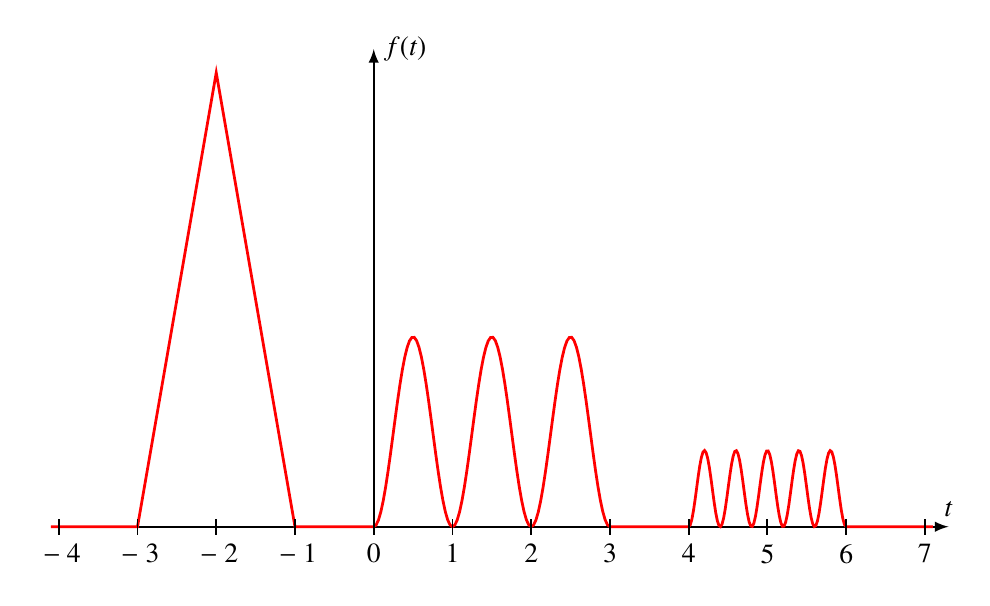
\begin{tikzpicture}[>=latex]

\draw[->,line width=0.7pt] (-4.1,0)--(7.3,0) coordinate[label={$t$}];
\draw[->,line width=0.7pt] (0,-0.1)--(0,{2*2.883+0.3})
	coordinate[label={right:$f(t)$}];

\draw[line width=1pt,color=red] (-4.1,0)--(-3,0)--(-2,{2*2.883})--(-1,0)--(0,0)--
	plot[domain=0:3,samples=100] ({\x},{1.205*(1-cos(2*180*\x))})
	--(3,0)--(4,0)--
	plot[domain=4:6,samples=100] ({\x},{0.968*0.5*(1-cos(5*180*\x))})
	--(7.1,0);

\foreach \x in {-4,...,7}{
	\draw[line width=0.7pt] ({\x},-0.1)--({\x},0.1);
	\node at ({\x},-0.1) [below] {$\mathstrut\x$};
}

\end{tikzpicture}
\end{document}

